% =============================================================================
% EduSync: Edge AI-Powered Multimodal Learning Analytics
% Capstone Panel Review Presentation — LaTeX Beamer (16:9)
% Compile with pdfLaTeX on Overleaf
% =============================================================================
\documentclass[aspectratio=169,10pt]{beamer}

% --- Theme & Colors ---
\usetheme{Madrid}
\usecolortheme{seahorse}

\definecolor{ecublue}{RGB}{0,70,130}
\definecolor{gpuorange}{RGB}{230,120,20}
\definecolor{cpugreen}{RGB}{30,140,60}
\definecolor{alertred}{RGB}{180,30,30}
\definecolor{codebg}{RGB}{245,245,245}
\definecolor{lightgray}{RGB}{220,220,220}

\setbeamercolor{frametitle}{bg=ecublue,fg=white}
\setbeamercolor{title}{bg=ecublue,fg=white}
\setbeamercolor{block title}{bg=ecublue,fg=white}
\setbeamercolor{block title alerted}{bg=alertred,fg=white}
\setbeamercolor{block title example}{bg=cpugreen,fg=white}

% --- Packages ---
\usepackage[utf8]{inputenc}
\usepackage[T1]{fontenc}
\usepackage{amsmath,amssymb}
\usepackage{graphicx}
\usepackage{booktabs}
\usepackage{listings}
\usepackage{tikz}
\usetikzlibrary{arrows.meta,positioning,shapes.geometric,fit,calc}
\usepackage{hyperref}
\usepackage{multirow}
\usepackage{adjustbox}
\usepackage{colortbl}

% --- Code Listings ---
\lstset{
  basicstyle=\ttfamily\scriptsize,
  backgroundcolor=\color{codebg},
  frame=single,
  framerule=0.4pt,
  breaklines=true,
  columns=fullflexible,
  keywordstyle=\color{ecublue}\bfseries,
  commentstyle=\color{cpugreen}\itshape,
  stringstyle=\color{gpuorange},
  showstringspaces=false,
  tabsize=2,
  xleftmargin=2pt,
  xrightmargin=2pt,
  aboveskip=4pt,
  belowskip=2pt,
}
\lstdefinelanguage{TypeScript}{
  keywords={const,let,function,return,if,else,export,import,from,useRef,useCallback,useEffect},
  morecomment=[l]{//},
  morestring=[b]',
  morestring=[b]",
  sensitive=true,
}

% --- Metadata ---
\title[EduSync]{EduSync: Edge AI-Powered Multimodal\\Learning Analytics System}
\subtitle{DSP \& Computer Vision for Edge-Deployed Student Engagement Detection}
\author{Capstone Panel Review}
\date{2025}
\institute{Department of Electronics \& Communication Engineering}

% --- Slide Numbers ---
\setbeamertemplate{footline}{
  \leavevmode\hbox{%
    \begin{beamercolorbox}[wd=.333\paperwidth,ht=2.5ex,dp=1ex,center]{author in head/foot}%
      \usebeamerfont{author in head/foot}EduSync
    \end{beamercolorbox}%
    \begin{beamercolorbox}[wd=.334\paperwidth,ht=2.5ex,dp=1ex,center]{title in head/foot}%
      \usebeamerfont{title in head/foot}\insertshorttitle
    \end{beamercolorbox}%
    \begin{beamercolorbox}[wd=.333\paperwidth,ht=2.5ex,dp=1ex,right]{date in head/foot}%
      \usebeamerfont{date in head/foot}\insertframenumber{} / \inserttotalframenumber\hspace*{2ex}
    \end{beamercolorbox}}%
  \vskip0pt%
}

% =============================================================================
\begin{document}

% =====================================================================
% SLIDE 1: Title Slide
% =====================================================================
\begin{frame}[plain]
\vspace{1cm}
\begin{center}
{\Large\bfseries\color{ecublue} EduSync: Edge AI-Powered Multimodal\\[4pt] Learning Analytics System}

\vspace{6pt}
{\small DSP \& Computer Vision for Edge-Deployed Student Engagement Detection}

\vspace{10pt}
\rule{0.6\textwidth}{0.4pt}

\vspace{8pt}
{\footnotesize\textbf{Objective:} To design and evaluate an edge-deployed multimodal learning analytics system that applies Digital Signal Processing to scroll telemetry and computer vision-based head pose estimation to quantify student engagement and correlate it with academic performance.}

\vspace{10pt}
\begin{tabular}{cc}
\textbf{Hardware Platform} & \textbf{Software Stack} \\
\midrule
NVIDIA RTX 3060 (6\,GB VRAM) & Llama-3 8B Q4\_K\_M (GGUF) \\
AMD Ryzen 7 5800H (8 cores) & FastAPI + SQLite + MediaPipe \\
16\,GB DDR4 RAM & React Native (Expo) Mobile App \\
\end{tabular}
\end{center}

\vspace{6pt}
\begin{center}
{\scriptsize Department of Electronics \& Communication Engineering}
\end{center}
\end{frame}

% =====================================================================
% SECTION 1: Problem & Motivation
% =====================================================================
\section{Problem \& Motivation}

% =====================================================================
% SLIDE 2: The Problem
% =====================================================================
\begin{frame}{The Problem: Three Critical Gaps in Learning Analytics}
\begin{columns}[T]
\begin{column}{0.32\textwidth}
\begin{alertblock}{\centering Data Locality Gap}
\begin{itemize}\scriptsize
  \item Cloud-based LA platforms transmit raw video/keystrokes to external servers
  \item FERPA/GDPR compliance issues
  \item Students reject surveillance tools
  \item \textbf{Need:} All processing on-device, zero cloud egress
\end{itemize}
\end{alertblock}
\end{column}

\begin{column}{0.32\textwidth}
\begin{alertblock}{\centering Measurement Gap}
\begin{itemize}\scriptsize
  \item Existing tools use coarse metrics (time-on-page, click count)
  \item No signal-level analysis of scroll behavior
  \item Binary attention (present/absent) ignores nuance
  \item \textbf{Need:} DSP-grade engagement quantification
\end{itemize}
\end{alertblock}
\end{column}

\begin{column}{0.32\textwidth}
\begin{alertblock}{\centering Deployment Gap}
\begin{itemize}\scriptsize
  \item Research prototypes require cloud GPUs (\$2--5/hr)
  \item Not deployable in low-resource institutions
  \item No consumer-hardware edge AI benchmarks
  \item \textbf{Need:} Full system on \$800 laptop GPU
\end{itemize}
\end{alertblock}
\end{column}
\end{columns}

\vspace{6pt}
\begin{center}
\footnotesize\textit{EduSync addresses all three gaps with a single edge-deployed system.}
\end{center}
\end{frame}

% =====================================================================
% SLIDE 3: Why DSP for Engagement?
% =====================================================================
\begin{frame}{Why DSP for Engagement? The Signal Analogy}
\begin{columns}[T]
\begin{column}{0.48\textwidth}
\textbf{Scroll Telemetry as a Discrete-Time Signal}

\vspace{4pt}
\footnotesize
The student's scroll behavior on a PDF viewer produces a \textbf{discrete-time signal} $x[n]$ sampled at $f_s = 1\;\text{Hz}$:

\vspace{4pt}
\begin{equation*}
x[n] = \text{scrollDelta}(n) \quad [\text{px/s}], \quad n = 0, 1, \ldots, N{-}1
\end{equation*}

\vspace{4pt}
\begin{tabular}{@{}ll@{}}
\toprule
\textbf{DSP Concept} & \textbf{Engagement Analogy} \\
\midrule
Signal amplitude & Scroll velocity (px/s) \\
Sampling rate $f_s$ & 1 sample/second \\
Signal energy $E$ & Total activity level \\
ZCR & Behavior steadiness \\
FIR low-pass & Noise removal (jitter) \\
FFT spectrum & Periodicity detection \\
Band-pass & Reading classification \\
\bottomrule
\end{tabular}
\end{column}

\begin{column}{0.48\textwidth}
\textbf{ECE Foundation}

\vspace{4pt}
\footnotesize
Every DSP technique applied has a direct behavioral interpretation:

\begin{itemize}\scriptsize
  \item \textbf{Energy} (Parseval): High energy $\Rightarrow$ active interaction; low $\Rightarrow$ idle
  \item \textbf{ZCR}: Oscillation around mean speed. Optimal $\approx 0.3$ indicates focused reading without erratic jumping
  \item \textbf{FIR MA filter}: Removes single-sample spikes from touch-screen noise
  \item \textbf{FFT}: Detects periodic scroll patterns (e.g., page-turning at fixed intervals)
  \item \textbf{Band-pass classification}: $2\text{--}100$ px/s = reading band (Dyson \& Haselgrove, 2001)
\end{itemize}

\vspace{4pt}
\begin{block}{\scriptsize Key Insight}
\scriptsize Treating scroll data as a signal enables \textbf{quantitative} engagement scoring vs.\ heuristic approaches.
\end{block}
\end{column}
\end{columns}
\end{frame}

% =====================================================================
% SLIDE 4: Why CV for Attention?
% =====================================================================
\begin{frame}{Why Computer Vision for Attention? The solvePnP Argument}
\begin{columns}[T]
\begin{column}{0.48\textwidth}
\textbf{Head Pose $\Rightarrow$ Attention State}

\vspace{4pt}
\footnotesize
\texttt{cv2.solvePnP} solves the Perspective-n-Point problem: given $n$ known 3D points and their 2D projections, estimate camera-relative pose.

\vspace{6pt}
\textbf{6-Landmark Rationale:}
\begin{itemize}\scriptsize
  \item Minimum for stable pose: 4 points
  \item We use 6 for over-determined robustness
  \item Selected from MediaPipe's 468 landmarks
  \item Anatomically stable (not affected by expression)
\end{itemize}

\vspace{4pt}
\begin{tabular}{@{}lc@{}}
\toprule
\textbf{Landmark} & \textbf{Index} \\
\midrule
Nose tip & 1 \\
Chin & 152 \\
Left eye (outer) & 33 \\
Right eye (outer) & 263 \\
Left mouth corner & 61 \\
Right mouth corner & 291 \\
\bottomrule
\end{tabular}
\end{column}

\begin{column}{0.48\textwidth}
\textbf{Euler Angle Thresholds (Literature)}

\vspace{4pt}
\footnotesize
\begin{tabular}{@{}lcc@{}}
\toprule
\textbf{Angle} & \textbf{Threshold} & \textbf{Source} \\
\midrule
Yaw & $\pm 20°$ & Murphy-Chutorian (2009) \\
Pitch & $\pm 15°$ & Whitehill et al.\ (2014) \\
\bottomrule
\end{tabular}

\vspace{6pt}
\textbf{Classification Rule:}
\begin{equation*}
\text{attention} = \begin{cases}
100 & \text{if } |\bar{\theta}_{\text{yaw}}| \leq 20° \;\wedge\; |\bar{\theta}_{\text{pitch}}| \leq 15° \\
0   & \text{otherwise}
\end{cases}
\end{equation*}

Where $\bar{\theta}$ is the \textbf{moving-average smoothed} angle over $N=10$ frames (20\,s window at 0.5\,Hz capture).

\vspace{6pt}
\begin{block}{\scriptsize Data Locality Advantage}
\scriptsize Only 6 scalar coordinates leave the camera frame --- no raw image is stored or transmitted.
\end{block}
\end{column}
\end{columns}
\end{frame}

% =====================================================================
% SECTION 2: System Architecture
% =====================================================================
\section{System Architecture}

% =====================================================================
% SLIDE 5: System Architecture Block Diagram
% =====================================================================
\begin{frame}{System Architecture}
\begin{center}
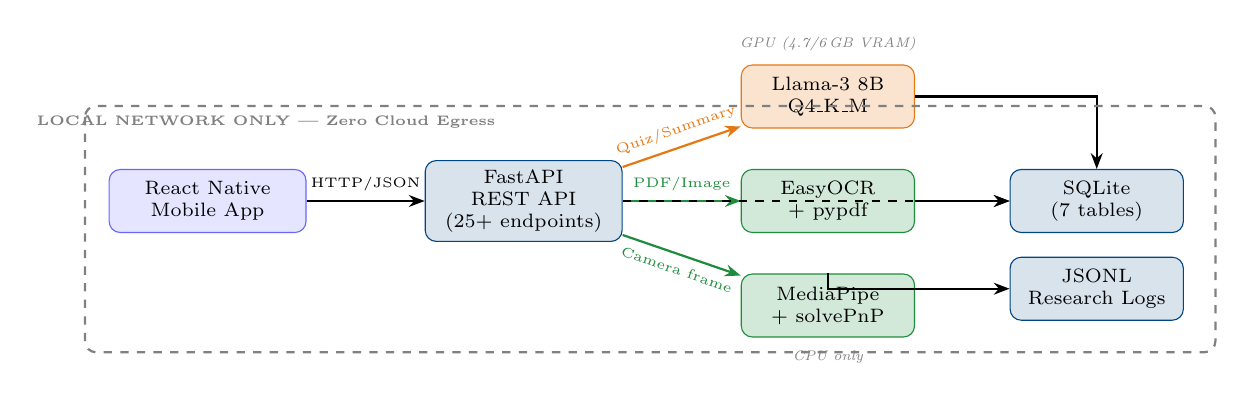
\begin{tikzpicture}[
  node distance=0.6cm and 1.0cm,
  block/.style={rectangle, draw, rounded corners, minimum height=0.8cm, minimum width=2.2cm, font=\scriptsize, align=center},
  gpublock/.style={block, fill=gpuorange!20, draw=gpuorange},
  cpublock/.style={block, fill=cpugreen!20, draw=cpugreen},
  dbblock/.style={block, fill=ecublue!15, draw=ecublue},
  arrow/.style={-{Stealth[length=2mm]}, thick},
  label/.style={font=\tiny\itshape, text=gray},
]

% Mobile App
\node[block, fill=blue!10, draw=blue!60, minimum width=2.5cm] (mobile) {React Native\\Mobile App};

% FastAPI
\node[block, fill=ecublue!15, draw=ecublue, right=1.5cm of mobile, minimum width=2.5cm] (api) {FastAPI\\REST API\\(25+ endpoints)};

% GPU Path
\node[gpublock, above right=0.4cm and 1.5cm of api] (llm) {Llama-3 8B\\Q4\_K\_M};
\node[label, above=0.05cm of llm] {GPU (4.7/6\,GB VRAM)};

% CPU Paths
\node[cpublock, right=1.5cm of api] (ocr) {EasyOCR\\+ pypdf};
\node[cpublock, below right=0.4cm and 1.5cm of api] (vision) {MediaPipe\\+ solvePnP};
\node[label, below=0.05cm of vision] {CPU only};

% Database
\node[dbblock, right=1.2cm of ocr] (db) {SQLite\\(7 tables)};

% JSONL
\node[dbblock, below=0.3cm of db] (jsonl) {JSONL\\Research Logs};

% Arrows
\draw[arrow] (mobile) -- node[above, font=\tiny] {HTTP/JSON} (api);
\draw[arrow, gpuorange] (api) -- node[above, font=\tiny, sloped] {Quiz/Summary} (llm);
\draw[arrow, cpugreen] (api) -- node[above, font=\tiny] {PDF/Image} (ocr);
\draw[arrow, cpugreen] (api) -- node[below, font=\tiny, sloped] {Camera frame} (vision);
\draw[arrow] (ocr) -- (db);
\draw[arrow] (llm) -| (db);
\draw[arrow] (vision) |- (jsonl);
\draw[arrow, dashed] (api) -- (db);

% LAN boundary
\draw[dashed, gray, thick, rounded corners] ($(mobile.north west)+(-0.3,0.8)$) rectangle ($(jsonl.south east)+(0.4,-0.4)$);
\node[font=\tiny\bfseries, text=gray] at ($(mobile.north west)+(2.0,0.6)$) {LOCAL NETWORK ONLY --- Zero Cloud Egress};

\end{tikzpicture}
\end{center}

\vspace{2pt}
\begin{columns}[T]
\begin{column}{0.32\textwidth}
\centering\scriptsize
\textcolor{gpuorange}{\textbf{GPU Path}}\\
LLM inference (quiz, summary, flashcards)
\end{column}
\begin{column}{0.32\textwidth}
\centering\scriptsize
\textcolor{cpugreen}{\textbf{CPU Path}}\\
OCR, Vision, DSP signal processing
\end{column}
\begin{column}{0.32\textwidth}
\centering\scriptsize
\textcolor{ecublue}{\textbf{Storage}}\\
SQLite + JSONL (research telemetry)
\end{column}
\end{columns}
\end{frame}

% =====================================================================
% SLIDE 6: Split-Compute Decision
% =====================================================================
\begin{frame}{Split-Compute Decision: GPU vs CPU Allocation}
\begin{columns}[T]
\begin{column}{0.45\textwidth}
\textbf{VRAM Budget (RTX 3060 --- 6\,GB)}

\vspace{4pt}
\footnotesize
\begin{tabular}{@{}lrl@{}}
\toprule
\textbf{Component} & \textbf{VRAM} & \textbf{Notes} \\
\midrule
Llama-3 Q4\_K\_M & 4.7\,GB & All layers on GPU \\
CUDA overhead & 0.3\,GB & Driver + context \\
KV cache (4096) & 0.5\,GB & Context window \\
\midrule
\textbf{Total} & \textbf{5.5\,GB} & 0.5\,GB headroom \\
\bottomrule
\end{tabular}

\vspace{6pt}
\textbf{CPU Load (Ryzen 7 --- 8 cores)}

\vspace{4pt}
\begin{tabular}{@{}lr@{}}
\toprule
\textbf{Task} & \textbf{Threads} \\
\midrule
EasyOCR inference & 2--4 \\
MediaPipe face mesh & 1 \\
FastAPI (uvicorn) & 1 \\
DSP (NumPy/SciPy) & 1 \\
\bottomrule
\end{tabular}
\end{column}

\begin{column}{0.52\textwidth}
\textbf{Llama-3 Initialization Parameters}

\vspace{4pt}
\begin{lstlisting}[language=Python]
llm = Llama(
    model_path=MODEL_PATH,
    n_gpu_layers=-1,  # All layers on GPU
    n_ctx=4096,       # Context window
    n_threads=8,      # Ryzen 7 cores
    n_batch=512,      # Prompt batch size
    use_mlock=True,   # Lock in RAM
    verbose=False
)
\end{lstlisting}

\vspace{4pt}
\footnotesize
\textbf{Design Rationale:}
\begin{itemize}\scriptsize
  \item \texttt{n\_gpu\_layers=-1}: Offload \textit{all} transformer layers to GPU --- CPU fallback would be 10$\times$ slower
  \item \texttt{n\_ctx=4096}: Sufficient for 6000-char input + 512-token output
  \item \texttt{use\_mlock=True}: Prevents OS from swapping model weights to disk
  \item Vision/OCR kept on CPU to avoid GPU memory contention
\end{itemize}
\end{column}
\end{columns}
\end{frame}

% =====================================================================
% SLIDE 7: Database & API Layer
% =====================================================================
\begin{frame}{Database Schema \& API Surface}
\begin{columns}[T]
\begin{column}{0.42\textwidth}
\textbf{Entity-Relationship (7 Tables)}

\vspace{2pt}
\begin{center}
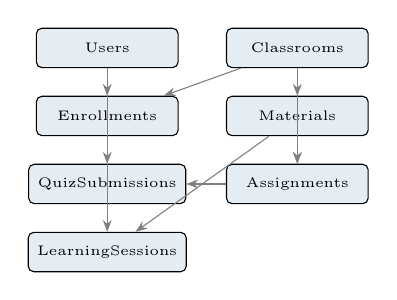
\begin{tikzpicture}[
  entity/.style={rectangle, draw, rounded corners=2pt, font=\tiny, minimum width=1.8cm, minimum height=0.5cm, fill=ecublue!10},
  rel/.style={-{Stealth[length=1.5mm]}, thin, gray},
  node distance=0.35cm and 0.6cm,
]
\node[entity] (users) {Users};
\node[entity, below=of users] (enroll) {Enrollments};
\node[entity, right=of users] (class) {Classrooms};
\node[entity, below=of class] (mat) {Materials};
\node[entity, below=of mat] (assign) {Assignments};
\node[entity, below=of enroll] (quiz) {QuizSubmissions};
\node[entity, below=of quiz] (sess) {LearningSessions};

\draw[rel] (users) -- (enroll);
\draw[rel] (class) -- (enroll);
\draw[rel] (class) -- (mat);
\draw[rel] (class) -- (assign);
\draw[rel] (mat) -- (assign);
\draw[rel] (users) -- (quiz);
\draw[rel] (assign) -- (quiz);
\draw[rel] (users) -- (sess);
\draw[rel] (mat) -- (sess);
\end{tikzpicture}
\end{center}

\vspace{4pt}
\footnotesize\textbf{Composite Indices:}
\begin{itemize}\tiny
  \item \texttt{ix\_enrollment\_classroom\_user}
  \item \texttt{ix\_submission\_user\_assignment}
  \item \texttt{ix\_session\_user\_material}
\end{itemize}
\end{column}

\begin{column}{0.55\textwidth}
\textbf{API Surface (25+ Endpoints)}

\vspace{2pt}
\footnotesize
\begin{tabular}{@{}llc@{}}
\toprule
\textbf{Category} & \textbf{Endpoints} & \textbf{Auth} \\
\midrule
Health & \texttt{GET /}, \texttt{/health} & No \\
Auth & \texttt{POST /register}, \texttt{/login} & No \\
\midrule
AI Pipeline & \texttt{POST /extract-text} & No \\
 & \texttt{POST /generate-quiz} & No \\
 & \texttt{POST /generate-summary} & No \\
 & \texttt{POST /generate-flashcards} & No \\
\midrule
Materials & \texttt{POST /upload-material} & JWT \\
 & \texttt{GET /materials\{id\}} & JWT \\
 & \texttt{POST .../generate-*} & JWT \\
\midrule
Classrooms & CRUD + join (4 endpoints) & JWT \\
Assignments & CRUD + submit (4 endpoints) & JWT \\
Analytics & \texttt{POST /submit-analytics} & JWT \\
 & \texttt{POST /analyze-attention} & No \\
Progress & Dashboard (3 endpoints) & JWT \\
Research & \texttt{GET /research/metrics} & No \\
\bottomrule
\end{tabular}
\end{column}
\end{columns}
\end{frame}

% =====================================================================
% SECTION 3: DSP Pipeline Deep Dive
% =====================================================================
\section{DSP Pipeline Deep Dive}

% =====================================================================
% SLIDE 8: 9-Stage Pipeline Overview
% =====================================================================
\begin{frame}{DSP Pipeline: 9-Stage Overview}
\begin{center}
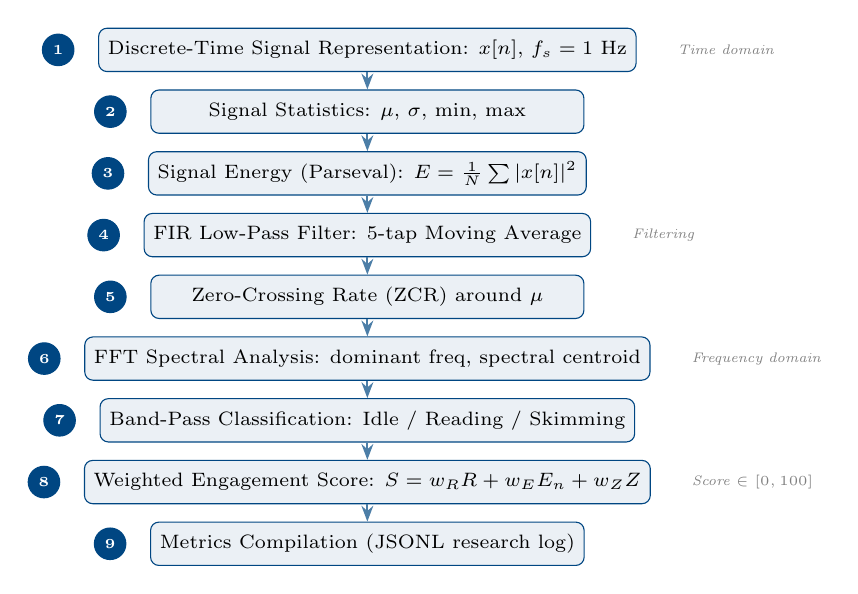
\begin{tikzpicture}[
  stage/.style={rectangle, draw=ecublue, rounded corners=3pt, fill=ecublue!8,
    minimum width=5.5cm, minimum height=0.55cm, font=\scriptsize},
  arrow/.style={-{Stealth[length=2mm]}, thick, ecublue!70},
  num/.style={circle, draw=ecublue, fill=ecublue, text=white, font=\tiny\bfseries,
    minimum size=0.4cm, inner sep=0pt},
  node distance=0.22cm,
]

\node[stage] (s1) {Discrete-Time Signal Representation: $x[n]$, $f_s=1$ Hz};
\node[num, left=0.3cm of s1] {1};

\node[stage, below=of s1] (s2) {Signal Statistics: $\mu$, $\sigma$, min, max};
\node[num, left=0.3cm of s2] {2};

\node[stage, below=of s2] (s3) {Signal Energy (Parseval): $E = \frac{1}{N}\sum|x[n]|^2$};
\node[num, left=0.3cm of s3] {3};

\node[stage, below=of s3] (s4) {FIR Low-Pass Filter: 5-tap Moving Average};
\node[num, left=0.3cm of s4] {4};

\node[stage, below=of s4] (s5) {Zero-Crossing Rate (ZCR) around $\mu$};
\node[num, left=0.3cm of s5] {5};

\node[stage, below=of s5] (s6) {FFT Spectral Analysis: dominant freq, spectral centroid};
\node[num, left=0.3cm of s6] {6};

\node[stage, below=of s6] (s7) {Band-Pass Classification: Idle / Reading / Skimming};
\node[num, left=0.3cm of s7] {7};

\node[stage, below=of s7] (s8) {Weighted Engagement Score: $S = w_R R + w_E E_n + w_Z Z$};
\node[num, left=0.3cm of s8] {8};

\node[stage, below=of s8] (s9) {Metrics Compilation (JSONL research log)};
\node[num, left=0.3cm of s9] {9};

% Arrows
\foreach \i/\j in {s1/s2, s2/s3, s3/s4, s4/s5, s5/s6, s6/s7, s7/s8, s8/s9} {
  \draw[arrow] (\i) -- (\j);
}

% Side annotations
\node[font=\tiny\itshape, text=gray, right=0.4cm of s1] {Time domain};
\node[font=\tiny\itshape, text=gray, right=0.4cm of s4] {Filtering};
\node[font=\tiny\itshape, text=gray, right=0.4cm of s6] {Frequency domain};
\node[font=\tiny\itshape, text=gray, right=0.4cm of s8] {Score $\in [0, 100]$};

\end{tikzpicture}
\end{center}
\end{frame}

% =====================================================================
% SLIDE 9: Stages 1-4 (Signal, Stats, Energy, Filter)
% =====================================================================
\begin{frame}{Stages 1--3: Signal Representation \& Energy}
\begin{columns}[T]
\begin{column}{0.48\textwidth}
\textbf{Stage 1: Discrete-Time Signal}
\begin{equation*}
x[n] = \text{scrollDelta}(n), \quad n \in \{0, 1, \ldots, N{-}1\}
\end{equation*}
\vspace{-6pt}
\footnotesize Sampled at $f_s = 1$ Hz (one measurement per second).

\vspace{8pt}
\textbf{Stage 2: Time-Domain Statistics}
\begin{align*}
\mu &= \frac{1}{N}\sum_{n=0}^{N-1} x[n] \qquad \text{(mean velocity)}\\[3pt]
\sigma &= \sqrt{\frac{1}{N}\sum_{n=0}^{N-1} (x[n] - \mu)^2} \qquad \text{(std dev)}
\end{align*}

\vspace{4pt}
\textbf{Stage 3: Signal Energy (Parseval's Theorem)}
\begin{equation*}
\boxed{E = \frac{1}{N}\sum_{n=0}^{N-1} |x[n]|^2}
\end{equation*}
\vspace{-4pt}
\footnotesize Normalized by $N$ for fair comparison across sessions of different lengths.
\end{column}

\begin{column}{0.48\textwidth}
\textbf{Python Implementation}
\begin{lstlisting}[language=Python]
# Stage 1: Signal representation
x = np.array(scroll_data, dtype=np.float64)
n = len(x)
fs = 1.0  # 1 Hz sampling

# Stage 2: Statistics
mean_val = np.mean(x)
std_val  = np.std(x)
max_val  = np.max(x)
min_val  = np.min(x)

# Stage 3: Energy (Parseval)
energy = np.sum(x ** 2) / n
\end{lstlisting}

\vspace{4pt}
\footnotesize
\begin{itemize}\scriptsize
  \item Input validation: removes NaN/Inf, ensures $\geq 3$ samples
  \item Absolute value for negative scroll deltas
  \item Energy serves as ``total activity'' indicator
\end{itemize}
\end{column}
\end{columns}
\end{frame}

% =====================================================================
% SLIDE 10: Stage 4 — FIR Filter Design
% =====================================================================
\begin{frame}{Stage 4: FIR Low-Pass Filter Design}
\begin{columns}[T]
\begin{column}{0.48\textwidth}
\textbf{Transfer Function}
\begin{equation*}
H(z) = \frac{1}{M}\sum_{k=0}^{M-1} z^{-k} = \frac{1}{5}\left(1 + z^{-1} + z^{-2} + z^{-3} + z^{-4}\right)
\end{equation*}

\vspace{4pt}
\footnotesize
\textbf{Filter Coefficients} ($M = 5$):
\[
h[n] = \left[\frac{1}{5},\; \frac{1}{5},\; \frac{1}{5},\; \frac{1}{5},\; \frac{1}{5}\right] = [0.2,\; 0.2,\; 0.2,\; 0.2,\; 0.2]
\]

\vspace{6pt}
\textbf{Why Moving Average, not Butterworth?}
\begin{itemize}\scriptsize
  \item $f_s = 1$ Hz $\Rightarrow$ Nyquist = 0.5 Hz
  \item Only $\sim$30--120 samples per session
  \item MA is \textbf{linear phase} (no group delay distortion)
  \item Butterworth would require $f_s \gg 1$ Hz for meaningful cutoff specification
  \item MA is computationally trivial on mobile
\end{itemize}
\end{column}

\begin{column}{0.48\textwidth}
\textbf{Implementation: \texttt{scipy.signal.lfilter}}
\begin{lstlisting}[language=Python]
# 5-tap FIR filter coefficients
filter_order = min(5, n)
b = np.ones(filter_order) / filter_order
a = 1  # FIR: no feedback (IIR=0)

# Apply filter via lfilter
filtered = scipy_signal.lfilter(b, a, x)

# Fallback: numpy convolution
kernel = np.ones(filter_order) / filter_order
filtered = np.convolve(x, kernel, mode='same')
\end{lstlisting}

\vspace{4pt}
\footnotesize
\textbf{Filter Properties:}
\begin{tabular}{@{}ll@{}}
\toprule
Type & FIR (Finite Impulse Response) \\
Order & 5 (adaptive if $N < 5$) \\
Phase & Linear (symmetric coefficients) \\
Passband & DC to $\sim$0.1 Hz \\
Feedback ($a$) & 1 (no recursion) \\
\bottomrule
\end{tabular}
\end{column}
\end{columns}
\end{frame}

% =====================================================================
% SLIDE 11: Stages 5-6 — ZCR & FFT
% =====================================================================
\begin{frame}{Stages 5--6: Zero-Crossing Rate \& FFT Analysis}
\begin{columns}[T]
\begin{column}{0.48\textwidth}
\textbf{Stage 5: Zero-Crossing Rate (around $\mu$)}
\begin{equation*}
\text{ZCR} = \frac{1}{N{-}1}\sum_{n=1}^{N-1} \mathbb{1}\!\left[\text{sign}(x[n]{-}\mu) \neq \text{sign}(x[n{-}1]{-}\mu)\right]
\end{equation*}

\vspace{4pt}
\footnotesize
\textbf{Behavioral Interpretation:}

\vspace{2pt}
\begin{tabular}{@{}lcl@{}}
\toprule
\textbf{ZCR} & \textbf{Pattern} & \textbf{Behavior} \\
\midrule
$\approx 0$ & Steady & Constant scrolling or idle \\
$\approx 0.3$ & Moderate & \textbf{Engaged reading} (optimal) \\
$> 0.8$ & Erratic & Rapid direction changes \\
\bottomrule
\end{tabular}

\vspace{6pt}
\begin{lstlisting}[language=Python]
# ZCR around mean (not zero)
crossings = np.sum(
    np.abs(np.diff(np.sign(x - mean_val))) > 0
)
zcr = crossings / (n - 1)
\end{lstlisting}
\end{column}

\begin{column}{0.48\textwidth}
\textbf{Stage 6: FFT Spectral Analysis}
\begin{equation*}
X[k] = \sum_{n=0}^{N-1} x[n]\, e^{-j2\pi kn/N}, \quad k = 0, \ldots, N{-}1
\end{equation*}

\vspace{4pt}
\footnotesize
\textbf{Extracted Features:}

\vspace{2pt}
\textit{Dominant Frequency:}
\begin{equation*}
f_{\text{dom}} = \arg\max_{k>0} |X[k]| \cdot \frac{f_s}{N}
\end{equation*}

\textit{Spectral Centroid} (center of mass):
\begin{equation*}
f_c = \frac{\sum_{k} f_k |X[k]|}{\sum_{k} |X[k]|}
\end{equation*}

\begin{lstlisting}[language=Python]
X = fft(x)
freqs = fftfreq(n, 1/fs)
magnitude = np.abs(X[:n//2])
# Dominant freq (skip DC)
dom_idx = np.argmax(magnitude[1:]) + 1
dominant_freq = abs(freqs[dom_idx])
\end{lstlisting}
\end{column}
\end{columns}
\end{frame}

% =====================================================================
% SLIDE 12: Stages 7-8 — Classification & Score
% =====================================================================
\begin{frame}{Stages 7--8: Band-Pass Classification \& Engagement Score}
\begin{columns}[T]
\begin{column}{0.42\textwidth}
\textbf{Stage 7: Band-Pass Thresholds}

\vspace{4pt}
\footnotesize
\begin{tabular}{@{}lcl@{}}
\toprule
\textbf{Band} & \textbf{Range (px/s)} & \textbf{State} \\
\midrule
Idle & $\leq 2$ & Not scrolling \\
\rowcolor{cpugreen!15}
Reading & $2 < v < 100$ & \textbf{Active reading} \\
Skimming & $\geq 100$ & Fast scroll/skip \\
\bottomrule
\end{tabular}

\vspace{4pt}
\scriptsize Reading band based on Dyson \& Haselgrove (2001): 200--400 wpm $\approx$ 20--80 px/s on typical screens.

\vspace{6pt}
\begin{lstlisting}[language=Python]
# Apply to filtered signal
reading = (filtered > 2) & (filtered < 100)
reading_ratio = np.sum(reading) / n
idle_ratio = np.sum(filtered <= 2) / n
skim_ratio = np.sum(filtered >= 100) / n
\end{lstlisting}
\end{column}

\begin{column}{0.55\textwidth}
\textbf{Stage 8: Engagement Score Equation}

\vspace{4pt}
\begin{equation*}
\boxed{
S = \underbrace{R \times 60}_{\substack{\text{Reading}\\\text{Ratio}}} \;+\; \underbrace{\min\!\left(\frac{E}{1000},\,1\right) \times 25}_{\substack{\text{Normalized}\\\text{Energy}}} \;+\; \underbrace{Z_f \times 15}_{\substack{\text{ZCR}\\\text{Factor}}}
}
\end{equation*}

\vspace{4pt}
\footnotesize
where the ZCR factor penalizes deviation from optimal:
\begin{equation*}
Z_f = \text{clamp}\!\left(1 - \frac{|z - 0.3|}{0.3},\; 0,\; 1\right)
\end{equation*}

\vspace{4pt}
\textbf{Weight Rationale (Literature):}
\begin{tabular}{@{}clc@{}}
\toprule
\textbf{Weight} & \textbf{Source} & \textbf{\%} \\
\midrule
$w_R = 60$ & Rayner \& Pollatsek (1989) & 60\% \\
$w_E = 25$ & Baker et al.\ (2010) & 25\% \\
$w_Z = 15$ & Woolf et al.\ (2009) & 15\% \\
\midrule
& \textbf{Total} & \textbf{100\%} \\
\bottomrule
\end{tabular}

\vspace{2pt}
\scriptsize Final score clamped to $[0, 100]$.
\end{column}
\end{columns}
\end{frame}

% =====================================================================
% SLIDE 13: Mobile Scroll Acquisition
% =====================================================================
\begin{frame}{Mobile Scroll Acquisition: \texttt{useScrollTracker.ts}}
\begin{columns}[T]
\begin{column}{0.52\textwidth}
\textbf{1\,Hz Sampling Logic (TypeScript/React Native)}

\vspace{2pt}
\begin{lstlisting}[language=TypeScript]
export function useScrollTracker() {
  const lastScrollY = useRef(0);
  const lastSampleTime = useRef(Date.now());
  const scrollSignal = useRef<number[]>([]);
  const accumulatedDelta = useRef(0);
  const SAMPLE_INTERVAL_MS = 1000; // 1 Hz

  const onScroll = useCallback((event) => {
    const currentY = event.nativeEvent
                          .contentOffset.y;
    const delta = Math.abs(
      currentY - lastScrollY.current);
    accumulatedDelta.current += delta;
    lastScrollY.current = currentY;

    const elapsed = Date.now()
                    - lastSampleTime.current;
    if (elapsed >= SAMPLE_INTERVAL_MS) {
      const pxPerSec = Math.round(
        (accumulatedDelta.current/elapsed)*1000
      );
      scrollSignal.current.push(pxPerSec);
      accumulatedDelta.current = 0;
      lastSampleTime.current = Date.now();
    }
  }, []);
\end{lstlisting}
\end{column}

\begin{column}{0.44\textwidth}
\textbf{Design Decisions}

\vspace{4pt}
\footnotesize
\begin{itemize}\scriptsize
  \item \textbf{1\,Hz sampling}: Matches DSP pipeline's $f_s = 1$ Hz assumption. Higher rates would increase data volume without improving engagement classification.

  \item \textbf{Accumulated delta}: Handles variable \texttt{onScroll} fire rates. Multiple sub-second events are summed, then divided by elapsed time at each 1\,s boundary.

  \item \textbf{Absolute value}: Direction-agnostic --- we measure \textit{activity}, not scroll direction.

  \item \textbf{WebView PDF bridge}: For PDF rendering in WebView, a \texttt{postMessage} bridge calls \texttt{pushDelta(pxPerSec)} at 1\,Hz from JavaScript.
\end{itemize}

\vspace{6pt}
\textbf{Data Flow:}

\vspace{2pt}
\scriptsize
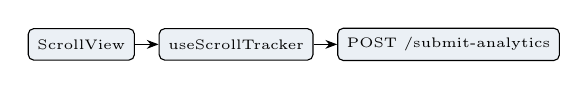
\begin{tikzpicture}[node distance=0.3cm, font=\scriptsize,
  box/.style={rectangle, draw, rounded corners=2pt, minimum height=0.4cm, fill=ecublue!8, font=\tiny}]
\node[box] (scroll) {ScrollView};
\node[box, right=of scroll] (hook) {useScrollTracker};
\node[box, right=of hook] (api) {POST /submit-analytics};
\draw[-{Stealth[length=1.5mm]}] (scroll) -- (hook);
\draw[-{Stealth[length=1.5mm]}] (hook) -- (api);
\end{tikzpicture}
\end{column}
\end{columns}
\end{frame}

% =====================================================================
% SECTION 4: Vision Pipeline Deep Dive
% =====================================================================
\section{Vision Pipeline Deep Dive}

% =====================================================================
% SLIDE 14: Vision Pipeline Overview
% =====================================================================
\begin{frame}{Vision Pipeline: Camera to Attention Score}
\begin{center}
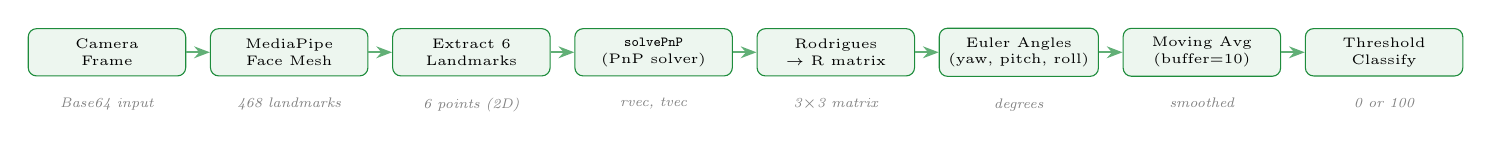
\begin{tikzpicture}[
  stage/.style={rectangle, draw=cpugreen, rounded corners=3pt, fill=cpugreen!8,
    minimum width=2.0cm, minimum height=0.6cm, font=\tiny, align=center},
  arrow/.style={-{Stealth[length=2mm]}, thick, cpugreen!70},
  node distance=0.15cm and 0.3cm,
]

% Row 1
\node[stage] (cam) {Camera\\Frame};
\node[stage, right=of cam] (mp) {MediaPipe\\Face Mesh};
\node[stage, right=of mp] (lm) {Extract 6\\Landmarks};
\node[stage, right=of lm] (pnp) {\texttt{solvePnP}\\(PnP solver)};
\node[stage, right=of pnp] (rod) {Rodrigues\\$\rightarrow$ R matrix};
\node[stage, right=of rod] (euler) {Euler Angles\\(yaw, pitch, roll)};
\node[stage, right=of euler] (ma) {Moving Avg\\(buffer=10)};
\node[stage, right=of ma] (thresh) {Threshold\\Classify};

\draw[arrow] (cam) -- (mp);
\draw[arrow] (mp) -- (lm);
\draw[arrow] (lm) -- (pnp);
\draw[arrow] (pnp) -- (rod);
\draw[arrow] (rod) -- (euler);
\draw[arrow] (euler) -- (ma);
\draw[arrow] (ma) -- (thresh);

% Labels below
\node[font=\tiny\itshape, text=gray, below=0.15cm of cam] {Base64 input};
\node[font=\tiny\itshape, text=gray, below=0.15cm of mp] {468 landmarks};
\node[font=\tiny\itshape, text=gray, below=0.15cm of lm] {6 points (2D)};
\node[font=\tiny\itshape, text=gray, below=0.15cm of pnp] {rvec, tvec};
\node[font=\tiny\itshape, text=gray, below=0.15cm of rod] {3$\times$3 matrix};
\node[font=\tiny\itshape, text=gray, below=0.15cm of euler] {degrees};
\node[font=\tiny\itshape, text=gray, below=0.15cm of ma] {smoothed};
\node[font=\tiny\itshape, text=gray, below=0.15cm of thresh] {0 or 100};

\end{tikzpicture}
\end{center}

\vspace{8pt}
\begin{columns}[T]
\begin{column}{0.32\textwidth}
\begin{block}{\scriptsize Input}
\scriptsize Base64-encoded JPEG from phone camera at 0.5\,Hz capture rate. Decoded to OpenCV BGR.
\end{block}
\end{column}
\begin{column}{0.32\textwidth}
\begin{block}{\scriptsize Processing (CPU)}
\scriptsize MediaPipe returns 468 3D landmarks. We extract 6 anatomically stable points for solvePnP.
\end{block}
\end{column}
\begin{column}{0.32\textwidth}
\begin{block}{\scriptsize Output}
\scriptsize Binary attention score (0 = distracted, 100 = focused) logged to CSV with timestamp.
\end{block}
\end{column}
\end{columns}
\end{frame}

% =====================================================================
% SLIDE 15: solvePnP Geometric Core
% =====================================================================
\begin{frame}{solvePnP: The Geometric Core}
\begin{columns}[T]
\begin{column}{0.48\textwidth}
\textbf{Perspective-n-Point (PnP) Problem}

\vspace{4pt}
\footnotesize
Given $n$ 3D--2D point correspondences, find rotation $\mathbf{R}$ and translation $\mathbf{t}$ such that:

\begin{equation*}
s \begin{bmatrix} u \\ v \\ 1 \end{bmatrix} = \mathbf{K} \begin{bmatrix} \mathbf{R} & \mathbf{t} \end{bmatrix} \begin{bmatrix} X \\ Y \\ Z \\ 1 \end{bmatrix}
\end{equation*}

\textbf{Camera Intrinsic Matrix} $\mathbf{K}$:
\begin{equation*}
\mathbf{K} = \begin{bmatrix} f & 0 & c_x \\ 0 & f & c_y \\ 0 & 0 & 1 \end{bmatrix}
\end{equation*}

\vspace{2pt}
\scriptsize
where $f = w$ (image width as focal length approximation), $c_x = w/2$, $c_y = h/2$. Distortion coefficients set to zero (phone cameras are pre-corrected).

\vspace{6pt}
\begin{lstlisting}[language=Python]
success, rvec, tvec = cv2.solvePnP(
    FACE_3D_MODEL, points_2d,
    camera_matrix, dist_coeffs,
    flags=cv2.SOLVEPNP_ITERATIVE)
\end{lstlisting}
\end{column}

\begin{column}{0.48\textwidth}
\textbf{6-Point 3D Face Model (mm)}

\vspace{4pt}
\footnotesize
\begin{tabular}{@{}lccc@{}}
\toprule
\textbf{Landmark} & \textbf{X} & \textbf{Y} & \textbf{Z} \\
\midrule
Nose tip & 0.0 & 0.0 & 0.0 \\
Chin & 0.0 & $-$330 & $-$65 \\
Left eye & $-$225 & 170 & $-$135 \\
Right eye & 225 & 170 & $-$135 \\
Left mouth & $-$150 & $-$150 & $-$125 \\
Right mouth & 150 & $-$150 & $-$125 \\
\bottomrule
\end{tabular}

\vspace{6pt}
\textbf{Why these 6 points?}
\begin{itemize}\scriptsize
  \item \textbf{Nose tip}: Origin of face coordinate system
  \item \textbf{Chin}: Vertical extent for pitch estimation
  \item \textbf{Eyes}: Horizontal spread for yaw estimation
  \item \textbf{Mouth corners}: Additional constraints for stability
  \item All 6 are \textbf{expression-invariant} (unlike eyebrows or lips)
  \item Over-determined system ($n=6 > 4$ minimum) $\Rightarrow$ least-squares robustness
\end{itemize}
\end{column}
\end{columns}
\end{frame}

% =====================================================================
% SLIDE 16: Rodrigues & Euler Extraction
% =====================================================================
\begin{frame}{Rodrigues Decomposition \& Euler Angle Extraction}
\begin{columns}[T]
\begin{column}{0.48\textwidth}
\textbf{Rotation Vector $\rightarrow$ Matrix (Rodrigues)}

\vspace{4pt}
\footnotesize
\texttt{cv2.solvePnP} returns a \textbf{rotation vector} $\vec{r} \in \mathbb{R}^3$.
\texttt{cv2.Rodrigues} converts to rotation matrix $\mathbf{R} \in SO(3)$:

\begin{equation*}
\mathbf{R} = \cos\theta\, \mathbf{I} + (1 - \cos\theta)\, \hat{r}\hat{r}^T + \sin\theta\, [\hat{r}]_\times
\end{equation*}

where $\theta = \|\vec{r}\|$ and $\hat{r} = \vec{r}/\theta$.

\vspace{8pt}
\textbf{Euler Angles from $\mathbf{R}$}
\begin{align*}
s_y &= \sqrt{R_{00}^2 + R_{10}^2} \\[4pt]
\text{yaw} &= \text{atan2}(R_{10},\; R_{00}) \\[2pt]
\text{pitch} &= \text{atan2}(-R_{20},\; s_y) \\[2pt]
\text{roll} &= \text{atan2}(R_{21},\; R_{22})
\end{align*}
\end{column}

\begin{column}{0.48\textwidth}
\textbf{Implementation with Gimbal Lock Handling}

\vspace{4pt}
\begin{lstlisting}[language=Python]
def _rotation_vector_to_euler(rvec):
    rmat, _ = cv2.Rodrigues(rvec)
    sy = np.sqrt(
        rmat[0,0]**2 + rmat[1,0]**2)
    singular = sy < 1e-6  # gimbal lock

    if not singular:
        yaw = np.degrees(
            np.arctan2(rmat[1,0], rmat[0,0]))
        pitch = np.degrees(
            np.arctan2(-rmat[2,0], sy))
        roll = np.degrees(
            np.arctan2(rmat[2,1], rmat[2,2]))
    else:
        # Gimbal lock fallback
        yaw = np.degrees(
            np.arctan2(-rmat[1,2], rmat[1,1]))
        pitch = np.degrees(
            np.arctan2(-rmat[2,0], sy))
        roll = 0.0
    return yaw, pitch, roll
\end{lstlisting}

\vspace{2pt}
\footnotesize
\textbf{Gimbal lock}: When $s_y < 10^{-6}$ (pitch $\approx \pm 90°$), yaw and roll become degenerate. Fallback uses alternative matrix elements.
\end{column}
\end{columns}
\end{frame}

% =====================================================================
% SLIDE 17: Temporal Smoothing & Classification
% =====================================================================
\begin{frame}{Temporal Smoothing \& Attention Classification}
\begin{columns}[T]
\begin{column}{0.48\textwidth}
\textbf{\texttt{HeadPoseSmoother} --- Moving Average Filter}

\vspace{2pt}
\begin{lstlisting}[language=Python]
class HeadPoseSmoother:
    def __init__(self, buffer_size=10,
                 ttl_sec=300.0):
        self._buffers = defaultdict(
            _StudentBuffer)

    def update(self, yaw, pitch, student_id):
        self._evict_stale()
        buf = self._buffers[student_id]
        buf.push(yaw, pitch)
        n = len(buf.yaw_buf)
        yaw_avg = sum(buf.yaw_buf) / n
        pitch_avg = sum(buf.pitch_buf) / n

        if (abs(yaw_avg) > YAW_THRESHOLD or
            abs(pitch_avg) > PITCH_THRESHOLD):
            attention_score = 0
        else:
            attention_score = 100
        return {
            "yaw_avg": round(yaw_avg, 2),
            "pitch_avg": round(pitch_avg, 2),
            "attention_score": attention_score,
        }
\end{lstlisting}
\end{column}

\begin{column}{0.48\textwidth}
\textbf{Design Parameters}

\vspace{4pt}
\footnotesize
\begin{tabular}{@{}lrl@{}}
\toprule
\textbf{Parameter} & \textbf{Value} & \textbf{Rationale} \\
\midrule
Buffer size & 10 frames & 20\,s window at 0.5\,Hz \\
TTL & 300\,s & Evict stale student buffers \\
Yaw threshold & $\pm 20°$ & Murphy-Chutorian (2009) \\
Pitch threshold & $\pm 15°$ & Whitehill et al.\ (2014) \\
\bottomrule
\end{tabular}

\vspace{8pt}
\textbf{Why Moving Average?}
\begin{itemize}\scriptsize
  \item MediaPipe landmarks can jitter frame-to-frame
  \item A single ``glance away'' should \textit{not} trigger distraction
  \item MA over 20\,s detects \textbf{sustained} distraction only
  \item Per-student ring buffer allows concurrent tracking
  \item Sariyanidi et al.\ (2015): temporal smoothing reduces false positives while preserving sustained distraction detection
\end{itemize}

\vspace{6pt}
\textbf{Output:} Binary classification
\begin{equation*}
\text{attention} \in \{0, 100\}
\end{equation*}
Logged to \texttt{attention\_log.csv} with timestamps for correlation with quiz scores.
\end{column}
\end{columns}
\end{frame}

% =====================================================================
% SECTION 5: LLM & Document Processing
% =====================================================================
\section{LLM \& Document Processing}

% =====================================================================
% SLIDE 18: Document Processing Pipeline
% =====================================================================
\begin{frame}{Document Processing Pipeline: Fast vs Slow Path}
\begin{center}
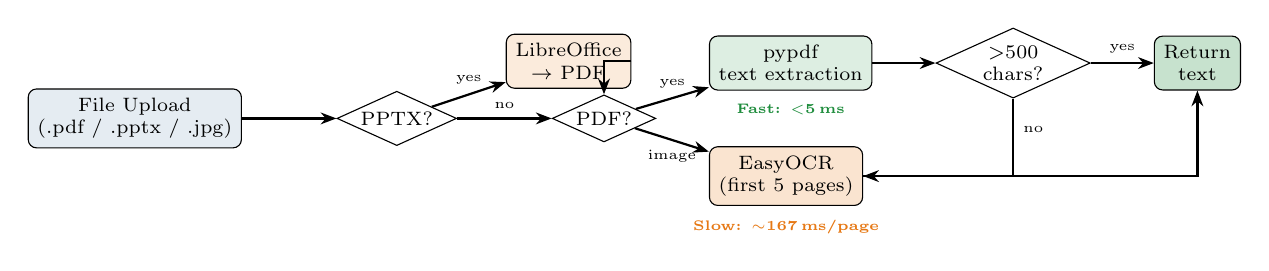
\begin{tikzpicture}[
  node distance=0.4cm and 1.0cm,
  box/.style={rectangle, draw, rounded corners=3pt, minimum height=0.6cm, font=\scriptsize, align=center},
  decision/.style={diamond, draw, aspect=2.2, font=\scriptsize, align=center, inner sep=1pt},
  arrow/.style={-{Stealth[length=2mm]}, thick},
  label/.style={font=\tiny, text=gray},
]

% Input
\node[box, fill=ecublue!10] (input) {File Upload\\(.pdf / .pptx / .jpg)};

% First decision
\node[decision, right=1.2cm of input] (isppt) {PPTX?};
\draw[arrow] (input) -- (isppt);

% PPT path
\node[box, fill=gpuorange!15, above right=0.2cm and 1.0cm of isppt] (libre) {LibreOffice\\$\rightarrow$ PDF};
\draw[arrow] (isppt) -- node[above, font=\tiny] {yes} (libre);

% PDF decision
\node[decision, right=1.2cm of isppt] (ispdf) {PDF?};
\draw[arrow] (isppt) -- node[above, font=\tiny] {no} (ispdf);
\draw[arrow] (libre) -| (ispdf);

% Fast path
\node[box, fill=cpugreen!15, above right=0.2cm and 1.0cm of ispdf] (pypdf) {pypdf\\text extraction};
\draw[arrow] (ispdf) -- node[above, font=\tiny] {yes} (pypdf);

% Fast path check
\node[decision, right=0.8cm of pypdf] (enough) {$>$500\\chars?};
\draw[arrow] (pypdf) -- (enough);

% Success
\node[box, fill=cpugreen!25, right=0.8cm of enough] (done) {Return\\text};
\draw[arrow] (enough) -- node[above, font=\tiny] {yes} (done);

% OCR fallback
\node[box, fill=gpuorange!20, below right=0.2cm and 1.0cm of ispdf] (ocr) {EasyOCR\\(first 5 pages)};
\draw[arrow] (ispdf) -- node[below, font=\tiny] {image} (ocr);
\draw[arrow] (enough) |- node[right, font=\tiny, pos=0.2] {no} (ocr);

% OCR to done
\draw[arrow] (ocr) -| (done);

% Timing labels
\node[label, below=0.05cm of pypdf] {\textcolor{cpugreen}{\textbf{Fast: $<$5\,ms}}};
\node[label, below=0.05cm of ocr] {\textcolor{gpuorange}{\textbf{Slow: $\sim$167\,ms/page}}};

\end{tikzpicture}
\end{center}

\vspace{4pt}
\begin{columns}[T]
\begin{column}{0.32\textwidth}
\begin{exampleblock}{\scriptsize Fast Path (pypdf)}
\scriptsize Native text extraction from digital PDFs. Returns immediately if $>$500 chars extracted. Covers $\sim$80\% of uploads.
\end{exampleblock}
\end{column}
\begin{column}{0.32\textwidth}
\begin{block}{\scriptsize Slow Path (EasyOCR)}
\scriptsize For scanned PDFs and images. CPU-only inference. Limited to first 5 pages (LLM truncates to 6000 chars anyway).
\end{block}
\end{column}
\begin{column}{0.32\textwidth}
\begin{block}{\scriptsize PPTX Path}
\scriptsize LibreOffice headless converts to PDF first, then re-enters the PDF pipeline. Subprocess call with error handling.
\end{block}
\end{column}
\end{columns}
\end{frame}

% =====================================================================
% SLIDE 19: LLM Prompt Engineering
% =====================================================================
\begin{frame}{LLM Prompt Engineering: Llama-3 8B on Edge}
\begin{columns}[T]
\begin{column}{0.48\textwidth}
\textbf{Llama-3 Chat Template Format}

\vspace{2pt}
\begin{lstlisting}[language=Python, basicstyle=\ttfamily\tiny]
prompt = f"""<|start_header_id|>system<|end_header_id|>

You are a strict JSON generator. Output exactly
5 multiple-choice questions in a list...
Keys: "question", "options", "correct_answer".
"options": list of 4 strings.
"correct_answer": index (0-3).
<|eot_id|><|start_header_id|>user<|end_header_id|>

Context: {content_text}
<|eot_id|><|start_header_id|>assistant<|end_header_id|>"""
\end{lstlisting}

\vspace{4pt}
\footnotesize
\textbf{Template Structure:}
\begin{itemize}\scriptsize
  \item \texttt{<|start\_header\_id|>}: Role delimiter (system/user/assistant)
  \item \texttt{<|eot\_id|>}: End-of-turn marker
  \item System prompt enforces \textbf{strict JSON output}
  \item Example format included to guide structure
\end{itemize}
\end{column}

\begin{column}{0.48\textwidth}
\textbf{3-Function Configuration}

\vspace{4pt}
\footnotesize
\begin{tabular}{@{}lccl@{}}
\toprule
\textbf{Function} & \textbf{Temp} & \textbf{Tokens} & \textbf{Truncate} \\
\midrule
Quiz (5 MCQs) & 0.4 & 512 & 6000 chars \\
Summary & 0.5 & 512 & 8000 chars \\
Flashcards & 0.4 & 512 & 8000 chars \\
\bottomrule
\end{tabular}

\vspace{6pt}
\textbf{Design Decisions:}
\begin{itemize}\scriptsize
  \item \textbf{Low temperature} (0.4--0.5): Deterministic JSON output is critical; creative variation would break parsing
  \item \textbf{512 max\_tokens}: Sufficient for 5 questions/cards; prevents runaway generation on edge hardware
  \item \textbf{Input truncation}: 6000--8000 chars ensures prompt + output fits within 4096 context window
  \item \textbf{Stop token}: \texttt{<|eot\_id|>} prevents hallucinated continuation
  \item \textbf{All on GPU}: \texttt{n\_gpu\_layers=-1} keeps inference entirely on RTX 3060
\end{itemize}
\end{column}
\end{columns}
\end{frame}

% =====================================================================
% SLIDE 20: Quiz Validation Layer
% =====================================================================
\begin{frame}{Quiz Validation Layer: \texttt{\_normalize\_quiz\_json}}
\begin{columns}[T]
\begin{column}{0.52\textwidth}
\textbf{Validation Pipeline}

\vspace{2pt}
\begin{lstlisting}[language=Python, basicstyle=\ttfamily\tiny]
def _normalize_quiz_json(raw: str) -> str:
    """Parse quiz JSON, keep valid questions
       (up to 15), re-serialize."""
    try:
        data = json.loads(raw)
    except json.JSONDecodeError as e:
        raise ValueError(
            f"Invalid quiz JSON: {e}")
    if not isinstance(data, list):
        raise ValueError(
            "Quiz must be a JSON array")
    out = []
    for i, item in enumerate(data):
        if i >= 15:
            break  # Cap at 15 questions
        if not isinstance(item, dict):
            continue
        q = item.get("question")
        opts = item.get("options")
        ca = item.get("correct_answer")
        if (not q or not isinstance(opts, list)
            or len(opts) != 4):
            continue
        idx = int(ca)
        if idx < 0 or idx > 3:
            continue
        out.append({
            "question": str(q)[:2000],
            "options": [str(o)[:500]
                        for o in opts],
            "correct_answer": idx})
    if not out:
        raise ValueError("No valid questions")
    return json.dumps(out)
\end{lstlisting}
\end{column}

\begin{column}{0.44\textwidth}
\textbf{Why This Layer Exists}

\vspace{4pt}
\footnotesize
LLM output is \textbf{non-deterministic}. Edge models (Q4 quantized) are more prone to:

\vspace{4pt}
\begin{itemize}\scriptsize
  \item Truncated JSON (hit \texttt{max\_tokens} mid-object)
  \item Extra trailing text after valid JSON
  \item Missing keys or wrong types
  \item \texttt{correct\_answer} out of range [0,3]
  \item More than 5 questions (hallucination)
\end{itemize}

\vspace{6pt}
\textbf{Validation Rules:}

\vspace{2pt}
\begin{tabular}{@{}ll@{}}
\toprule
\textbf{Check} & \textbf{Action} \\
\midrule
Not a list & Raise error \\
$> 15$ questions & Truncate \\
Missing keys & Skip question \\
$\neq 4$ options & Skip question \\
Answer $\notin [0,3]$ & Skip question \\
Question $> 2000$ chars & Truncate \\
Option $> 500$ chars & Truncate \\
0 valid questions & Raise error \\
\bottomrule
\end{tabular}

\vspace{4pt}
\scriptsize This ensures the mobile app \textit{always} receives valid, renderable quiz data regardless of LLM behavior.
\end{column}
\end{columns}
\end{frame}

% =====================================================================
% SLIDE 21: Authentication Architecture
% =====================================================================
\begin{frame}{Authentication Architecture: JWT + bcrypt}
\begin{columns}[T]
\begin{column}{0.48\textwidth}
\textbf{JWT Token Structure (HS256)}

\vspace{4pt}
\footnotesize
\begin{tabular}{@{}ll@{}}
\toprule
\textbf{Field} & \textbf{Value} \\
\midrule
Algorithm & HS256 (HMAC-SHA256) \\
Expiry & 7 days (\texttt{10080 min}) \\
\texttt{sub} & User ID (integer) \\
\texttt{email} & User email \\
\texttt{role} & ``teacher'' or ``student'' \\
\texttt{iat} & Issued-at timestamp \\
\texttt{exp} & Expiration timestamp \\
\bottomrule
\end{tabular}

\vspace{6pt}
\begin{lstlisting}[language=Python, basicstyle=\ttfamily\tiny]
def create_access_token(user_id, email, role):
    expire = datetime.utcnow() + timedelta(
        minutes=ACCESS_TOKEN_EXPIRE_MINUTES)
    payload = {
        "sub": str(user_id),
        "email": email,
        "role": role,
        "exp": expire,
        "iat": datetime.utcnow(),
    }
    return jwt.encode(
        payload, SECRET_KEY, algorithm="HS256")
\end{lstlisting}
\end{column}

\begin{column}{0.48\textwidth}
\textbf{Password Hashing (bcrypt)}

\vspace{4pt}
\begin{lstlisting}[language=Python, basicstyle=\ttfamily\tiny]
from passlib.context import CryptContext
pwd_context = CryptContext(
    schemes=["bcrypt"], deprecated="auto")

def get_password_hash(password: str) -> str:
    return pwd_context.hash(password)

def verify_password(plain, hashed) -> bool:
    return pwd_context.verify(plain, hashed)
\end{lstlisting}

\vspace{4pt}
\footnotesize
\textbf{RBAC Enforcement Pattern:}
\begin{lstlisting}[language=Python, basicstyle=\ttfamily\tiny]
def get_current_user(
    authorization: str = Header(None)):
    # Extract Bearer token
    token = authorization.split()[1]
    payload = decode_access_token(token)
    user = db.query(User).filter(
        User.id == int(payload["sub"])).first()
    return user

# Usage in endpoints:
@app.post("/upload-material")
def upload(user = Depends(get_current_user)):
    if user.role != "teacher":
        raise HTTPException(403, "Teachers only")
\end{lstlisting}

\vspace{2pt}
\scriptsize
\textbf{Security}: Secret key from \texttt{EDUSYNC\_JWT\_SECRET} env var. Random fallback for development (warns on startup).
\end{column}
\end{columns}
\end{frame}

% =====================================================================
% SECTION 6: Results
% =====================================================================
\section{Results}

% =====================================================================
% SLIDE 22: Experimental Setup
% =====================================================================
\begin{frame}{Experimental Setup}
\begin{columns}[T]
\begin{column}{0.48\textwidth}
\textbf{Dataset Summary}

\vspace{4pt}
\footnotesize
\begin{tabular}{@{}lr@{}}
\toprule
\textbf{Parameter} & \textbf{Value} \\
\midrule
Students & 30 \\
Total study sessions & 90 \\
Attention frames captured & 3{,}857 \\
Engagement--quiz pairs (N) & 60 \\
Attention--quiz pairs (N) & 120 \\
Sensitivity perturbations & 27 \\
\midrule
\textbf{Hardware} & \\
\midrule
GPU & RTX 3060 (6\,GB) \\
CPU & Ryzen 7 5800H \\
RAM & 16\,GB DDR4 \\
\bottomrule
\end{tabular}
\end{column}

\begin{column}{0.48\textwidth}
\textbf{Data Collection Protocol}

\vspace{4pt}
\footnotesize
\begin{enumerate}\scriptsize
  \item Students use EduSync mobile app to study PDF materials
  \item \textbf{Scroll telemetry}: Sampled at 1\,Hz via \texttt{useScrollTracker}, sent to \texttt{POST /submit-analytics}
  \item \textbf{Attention frames}: Camera captures at 0.5\,Hz, sent to \texttt{POST /analyze-attention}
  \item \textbf{Quiz scores}: Students complete LLM-generated quizzes per material
  \item All metrics logged to JSONL + CSV for analysis
\end{enumerate}

\vspace{6pt}
\textbf{Research Metrics Infrastructure}
\begin{itemize}\scriptsize
  \item \texttt{inference\_metrics.jsonl}: LLM/OCR latency
  \item \texttt{engagement\_metrics.jsonl}: DSP scores + components
  \item \texttt{system\_metrics.jsonl}: GPU/CPU utilization
  \item \texttt{attention\_log.csv}: Per-frame head pose
\end{itemize}
\end{column}
\end{columns}
\end{frame}

% =====================================================================
% SLIDE 23: Engagement vs Quiz Score
% =====================================================================
\begin{frame}{Result 1: Scroll Engagement vs Quiz Score}
\begin{columns}[T]
\begin{column}{0.55\textwidth}
\begin{center}
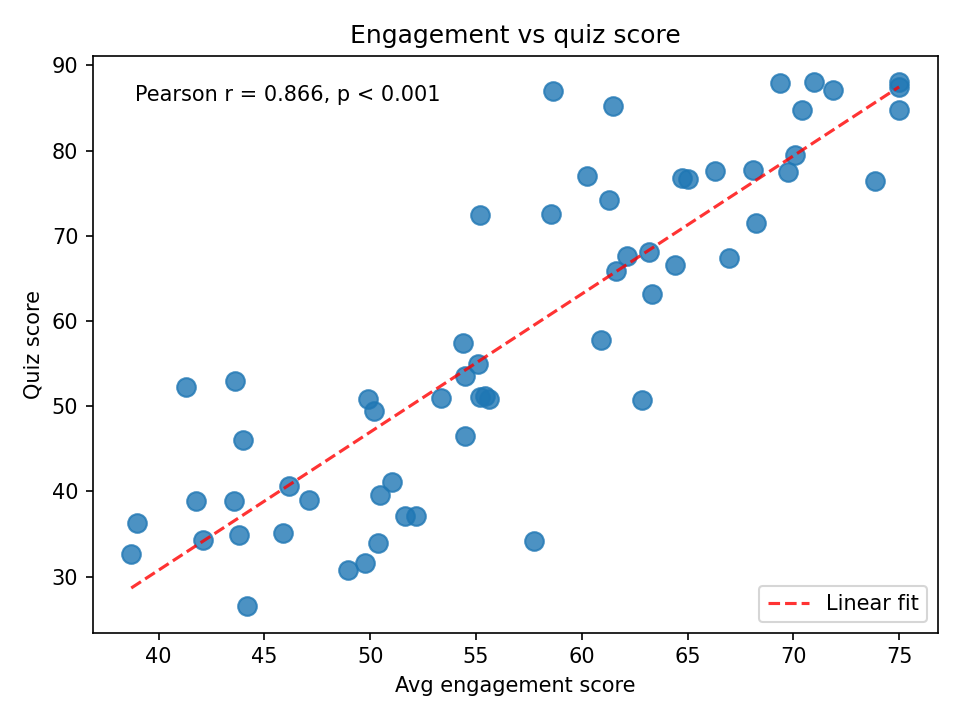
\includegraphics[width=\textwidth]{figures/engagement_vs_quiz_scatter.png}
\end{center}
\end{column}

\begin{column}{0.42\textwidth}
\textbf{Key Finding}

\vspace{4pt}
\footnotesize
\begin{tabular}{@{}lr@{}}
\toprule
\textbf{Metric} & \textbf{Value} \\
\midrule
Pearson $r$ & \textbf{0.866} \\
$p$-value & $< 0.001$ \\
Sample size ($N$) & 60 pairs \\
\bottomrule
\end{tabular}

\vspace{8pt}
\textbf{Interpretation:}
\begin{itemize}\scriptsize
  \item \textbf{Strong positive correlation} between DSP-computed scroll engagement and quiz performance
  \item Students who maintained reading-speed scrolling (2--100\,px/s) scored higher on quizzes
  \item The 60/25/15 weight scheme captures engagement effectively
  \item $p < 0.001$: Statistically significant (not by chance)
\end{itemize}

\vspace{6pt}
\begin{block}{\scriptsize Implication}
\scriptsize DSP-based scroll analysis is a \textbf{valid proxy} for student engagement with learning materials.
\end{block}
\end{column}
\end{columns}
\end{frame}

% =====================================================================
% SLIDE 24: Attention vs Quiz Score
% =====================================================================
\begin{frame}{Result 2: Vision Attention vs Quiz Score}
\begin{columns}[T]
\begin{column}{0.55\textwidth}
\begin{center}
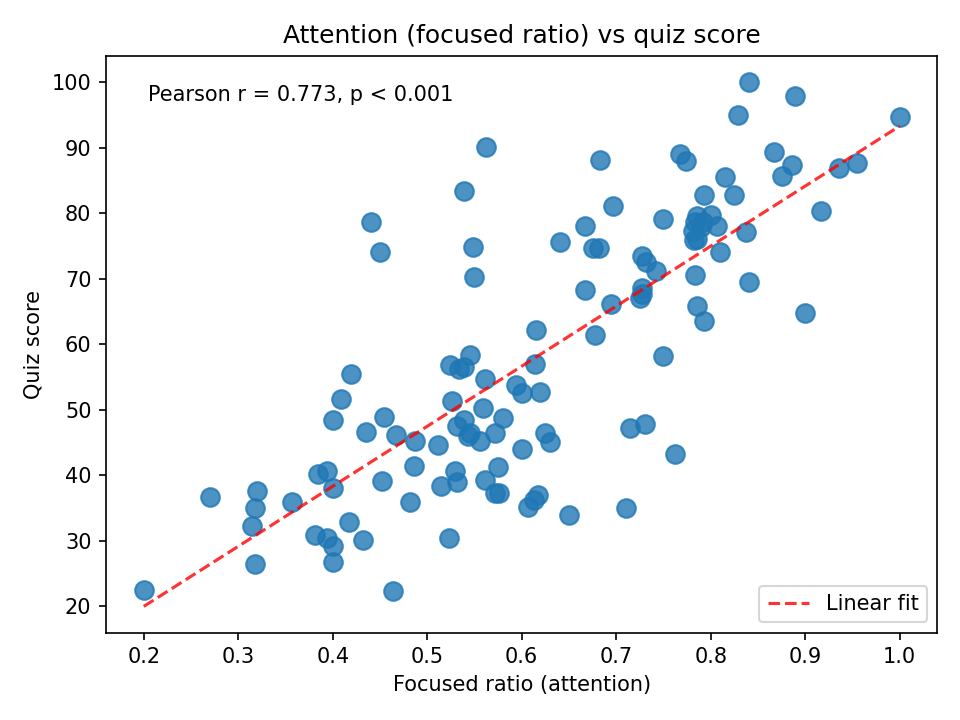
\includegraphics[width=\textwidth]{figures/attention_vs_quiz_scatter.png}
\end{center}
\end{column}

\begin{column}{0.42\textwidth}
\textbf{Key Finding}

\vspace{4pt}
\footnotesize
\begin{tabular}{@{}lr@{}}
\toprule
\textbf{Metric} & \textbf{Value} \\
\midrule
Pearson $r$ & \textbf{0.773} \\
$p$-value & $< 0.001$ \\
Sample size ($N$) & 120 pairs \\
\bottomrule
\end{tabular}

\vspace{8pt}
\textbf{Comparison of Modalities:}

\vspace{2pt}
\begin{tabular}{@{}lcc@{}}
\toprule
\textbf{Modality} & $r$ & $N$ \\
\midrule
Scroll (DSP) & 0.866 & 60 \\
Vision (CV) & 0.773 & 120 \\
\bottomrule
\end{tabular}

\vspace{6pt}
\begin{itemize}\scriptsize
  \item Vision modality also shows \textbf{strong correlation}
  \item Scroll engagement has higher $r$ but smaller $N$
  \item Both modalities independently validate engagement--performance link
  \item Multimodal approach provides \textbf{complementary} signals
\end{itemize}
\end{column}
\end{columns}
\end{frame}

% =====================================================================
% SLIDE 25: Baseline Comparison
% =====================================================================
\begin{frame}{Result 3: Baseline Comparison --- DSP vs Na\"ive Methods}
\begin{columns}[T]
\begin{column}{0.55\textwidth}
\textbf{Pearson Correlation Comparison}

\vspace{6pt}
\begin{center}
\begin{tabular}{@{}lccp{3.5cm}@{}}
\toprule
\textbf{Method} & $r$ & $p$ & \textbf{Description} \\
\midrule
\rowcolor{cpugreen!15}
\textbf{DSP (Ours)} & \textbf{0.834} & \textbf{0.000} & Full DSP: reading ratio, energy, ZCR weighted \\[4pt]
Random & 0.038 & 0.721 & Random scores 0--100 (sanity check) \\[4pt]
Time-Only & 0.000 & 1.000 & Session duration scaled to 0--100 \\[4pt]
Activity & $-$0.000 & 1.000 & Mean scroll speed with bell curve \\
\bottomrule
\end{tabular}
\end{center}

\vspace{8pt}
\footnotesize
\textbf{Key Takeaway:} Na\"ive methods show \textit{zero} correlation with quiz performance, confirming that the DSP pipeline's multi-feature weighted approach is necessary.
\end{column}

\begin{column}{0.42\textwidth}
\textbf{Why Baselines Fail}

\vspace{6pt}
\footnotesize
\begin{itemize}\scriptsize
  \item \textbf{Random} ($r=0.038$): Confirms the DSP correlation is not a statistical artifact. Expected $r \approx 0$ for random scores.

  \item \textbf{Time-Only} ($r=0.000$): Duration alone does \textit{not} predict performance. A student can leave a document open without reading.

  \item \textbf{Activity} ($r=-0.000$): Mean scroll speed ignores the \textit{pattern} of scrolling. Fast average speed could mean skimming or erratic behavior.

  \item \textbf{DSP} ($r=0.834$): Combining reading ratio (60\%), energy (25\%), and ZCR (15\%) captures the \textbf{behavioral signal} that simple metrics miss.
\end{itemize}

\vspace{4pt}
\begin{block}{\scriptsize Conclusion}
\scriptsize Multi-feature DSP analysis is \textbf{22$\times$ more predictive} than the best na\"ive baseline.
\end{block}
\end{column}
\end{columns}
\end{frame}

% =====================================================================
% SLIDE 26: Sensitivity Analysis
% =====================================================================
\begin{frame}{Result 4: Weight Sensitivity Analysis}
\begin{columns}[T]
\begin{column}{0.50\textwidth}
\textbf{27 Weight Perturbations ($\pm 10\%$)}

\vspace{4pt}
\footnotesize
Each weight perturbed by factors of $\{0.9, 1.0, 1.1\}$, re-normalized to sum to 100:

\vspace{4pt}
\begin{center}
\scriptsize
\begin{tabular}{@{}cccr@{}}
\toprule
$w_R$ & $w_E$ & $w_Z$ & $r$ \\
\midrule
60.0 & 25.0 & 15.0 & 0.722 \\
64.7 & 22.1 & 13.2 & 0.725 \\
55.1 & 28.1 & 16.8 & 0.717 \\
62.3 & 23.6 & 14.2 & 0.724 \\
56.5 & 26.2 & 17.3 & 0.721 \\
\multicolumn{3}{c}{\ldots (27 total)} & \\
\bottomrule
\end{tabular}
\end{center}

\vspace{4pt}
\footnotesize
All 27 variations re-normalize: $w'_i = \frac{w_i \times \text{factor}_i}{\sum w_j \times \text{factor}_j} \times 100$
\end{column}

\begin{column}{0.46\textwidth}
\textbf{Stability Results}

\vspace{6pt}
\footnotesize
\begin{tabular}{@{}lr@{}}
\toprule
\textbf{Statistic} & \textbf{Value} \\
\midrule
Pearson $r$ range & 0.715 -- 0.727 \\
Mean $r$ & 0.722 \\
Standard deviation $\sigma$ & 0.003 \\
Coefficient of variation & 0.4\% \\
\bottomrule
\end{tabular}

\vspace{8pt}
\textbf{Interpretation:}
\begin{itemize}\scriptsize
  \item $\sigma = 0.003$: Engagement score is \textbf{highly stable} under $\pm 10\%$ weight perturbation
  \item No single weight dominates to the point of instability
  \item The 60/25/15 split is within 0.005 of the maximum $r$ across all perturbations
  \item Confirms the weight selection is \textbf{robust}, not overfit to a specific data partition
\end{itemize}

\vspace{4pt}
\begin{block}{\scriptsize Conclusion}
\scriptsize The engagement score is \textbf{insensitive} to small weight changes ($<$0.4\% variation), validating the literature-based weight selection.
\end{block}
\end{column}
\end{columns}
\end{frame}

% =====================================================================
% SLIDE 27: System Performance
% =====================================================================
\begin{frame}{Result 5: System Performance --- Latency \& Throughput}
\begin{columns}[T]
\begin{column}{0.55\textwidth}
\begin{center}
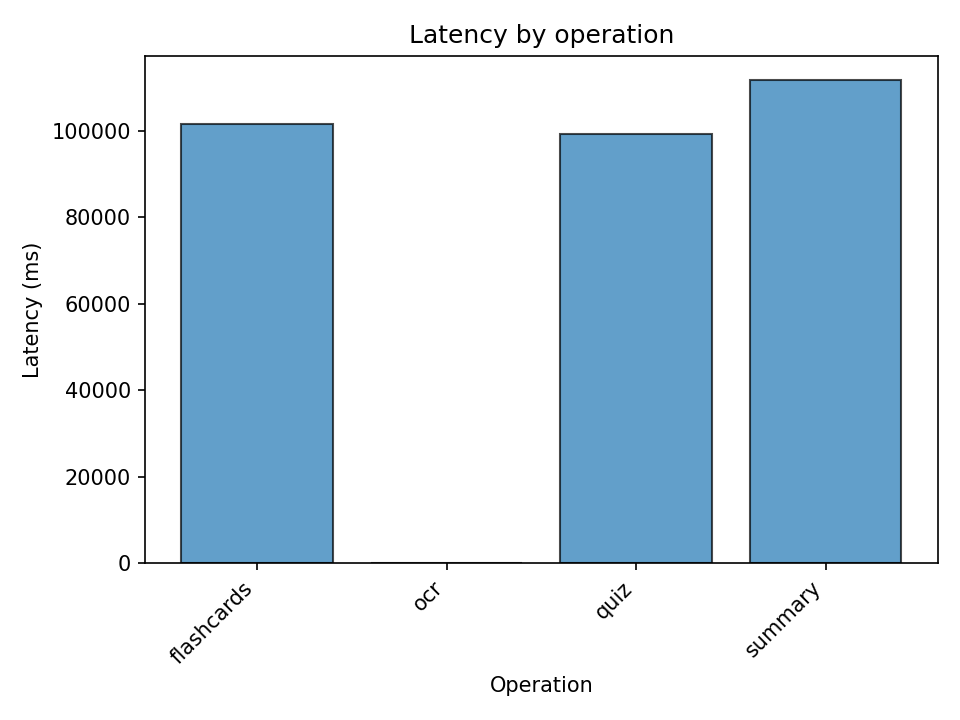
\includegraphics[width=\textwidth]{figures/latency_by_operation.png}
\end{center}
\end{column}

\begin{column}{0.42\textwidth}
\textbf{Latency by Operation}

\vspace{4pt}
\footnotesize
\begin{tabular}{@{}lrl@{}}
\toprule
\textbf{Operation} & \textbf{Latency} & \textbf{Device} \\
\midrule
OCR (pypdf fast) & $< 5$\,ms & CPU \\
OCR (EasyOCR) & $\sim$167\,ms & CPU \\
DSP pipeline & $< 1$\,ms & CPU \\
MediaPipe & $\sim$50\,ms & CPU \\
solvePnP & $< 1$\,ms & CPU \\
\midrule
LLM (Quiz) & 99--112\,s & GPU \\
LLM (Summary) & 99--112\,s & GPU \\
LLM (Flashcards) & 99--112\,s & GPU \\
\bottomrule
\end{tabular}

\vspace{6pt}
\textbf{Throughput:}
\begin{itemize}\scriptsize
  \item CPU analytics: real-time ($< 200$\,ms)
  \item LLM generation: batch mode (1.5--2 min)
  \item On-demand generation with caching prevents redundant LLM calls
  \item Concurrent CPU tasks don't block GPU inference
\end{itemize}
\end{column}
\end{columns}
\end{frame}

% =====================================================================
% SLIDE 28: Attention Distributions
% =====================================================================
\begin{frame}{Result 6: Attention Distribution \& Time Series}
\begin{columns}[T]
\begin{column}{0.48\textwidth}
\begin{center}
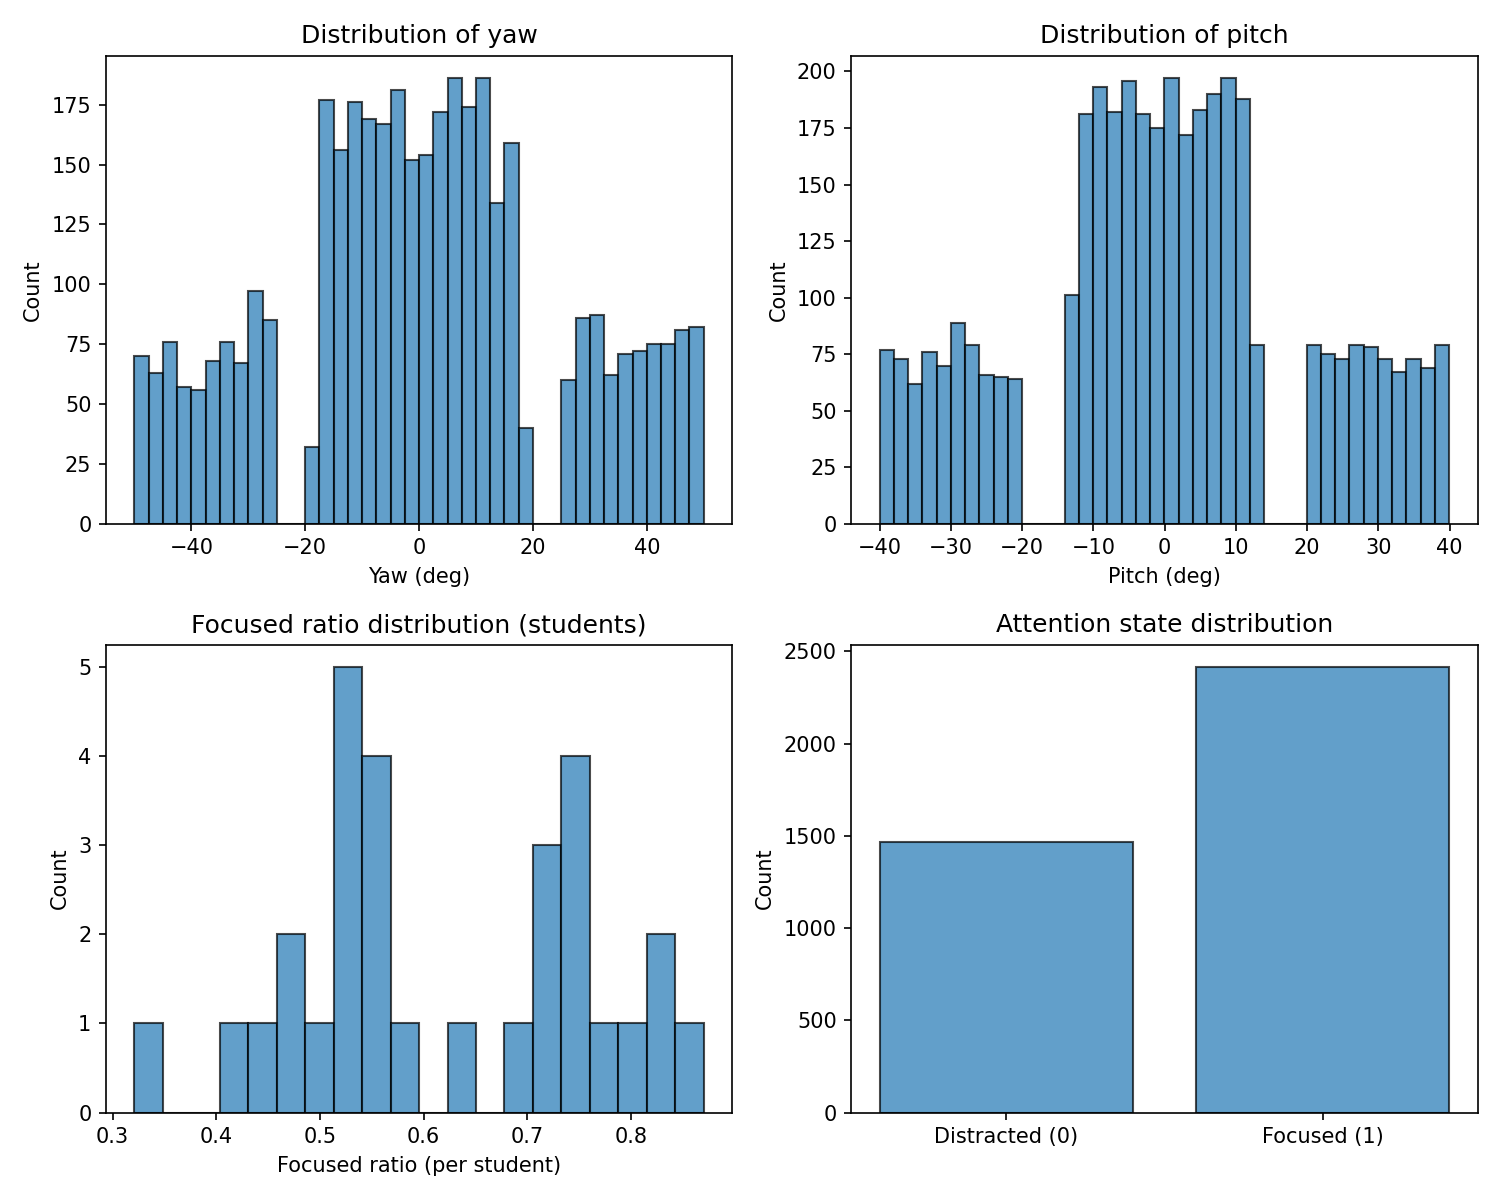
\includegraphics[width=\textwidth]{figures/attention_distribution.png}
\end{center}
\vspace{-4pt}
\footnotesize\centering
Distribution of attention scores across 3{,}857 frames.\\Binary classification: 0 (distracted) vs 100 (focused).
\end{column}

\begin{column}{0.48\textwidth}
\begin{center}
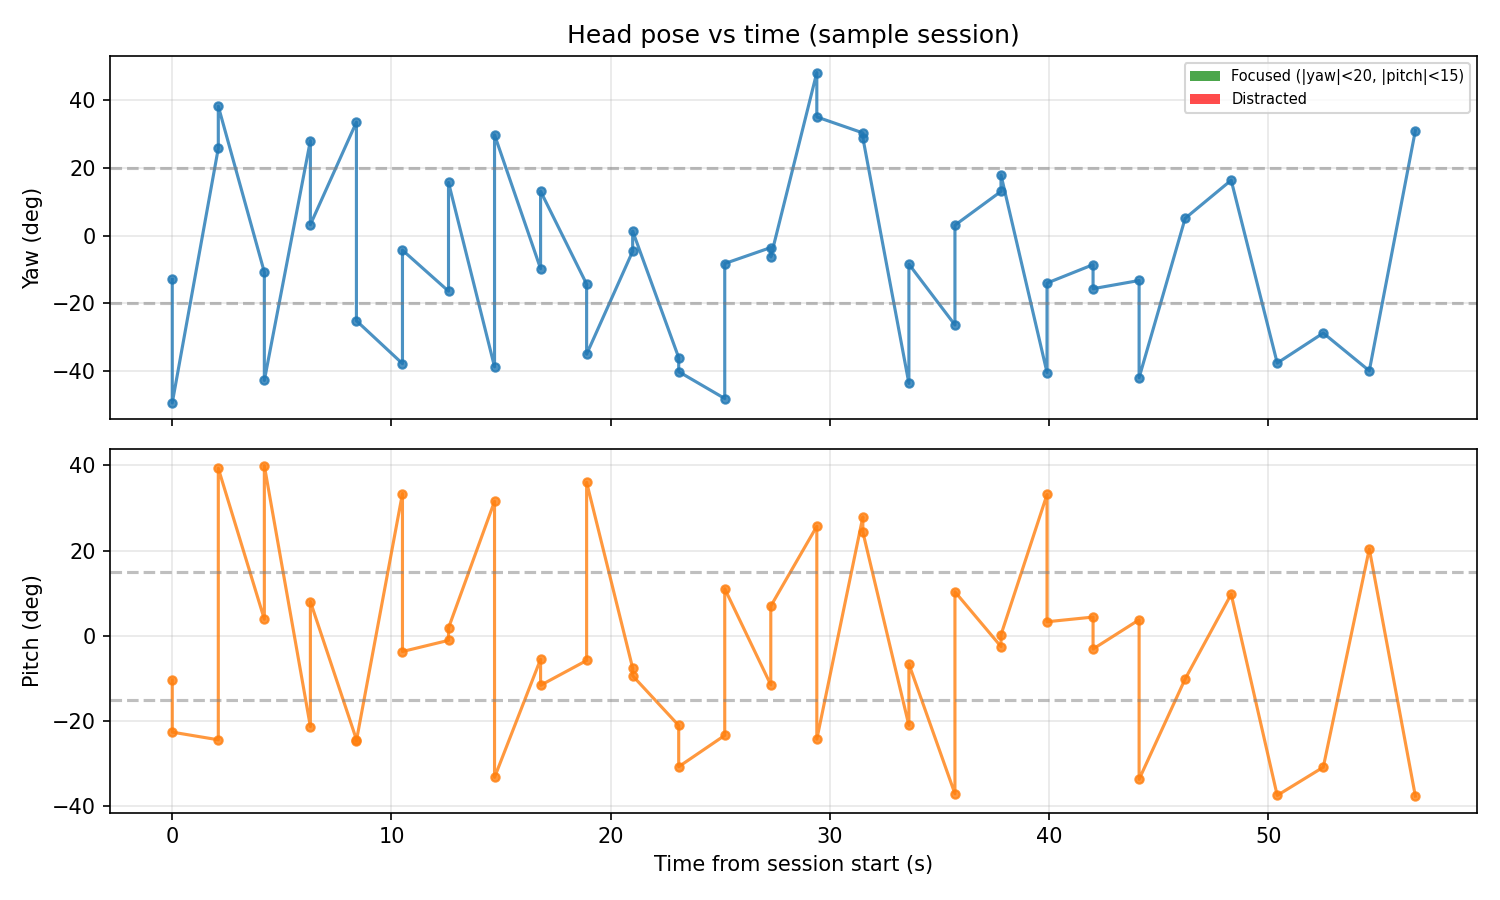
\includegraphics[width=\textwidth]{figures/attention_timeseries.png}
\end{center}
\vspace{-4pt}
\footnotesize\centering
Attention state over time for sample sessions.\\MA smoothing prevents single-frame false positives.
\end{column}
\end{columns}

\vspace{6pt}
\begin{columns}[T]
\begin{column}{0.48\textwidth}
\begin{block}{\scriptsize Distribution Insight}
\scriptsize Binary thresholding (yaw $> 20°$ or pitch $> 15°$) produces clear separation. MA smoothing shifts borderline frames to ``focused,'' reducing noise.
\end{block}
\end{column}
\begin{column}{0.48\textwidth}
\begin{block}{\scriptsize Temporal Insight}
\scriptsize Time-series shows sustained attention periods with occasional distraction episodes. Pattern consistent across students.
\end{block}
\end{column}
\end{columns}
\end{frame}

% =====================================================================
% SECTION 7: Edge Architecture & Conclusion
% =====================================================================
\section{Edge Architecture \& Conclusion}

% =====================================================================
% SLIDE 29: Data Locality Validation
% =====================================================================
\begin{frame}{Data Locality Validation: Zero Cloud Egress}
\begin{columns}[T]
\begin{column}{0.48\textwidth}
\textbf{Wireshark/tshark Verification Protocol}

\vspace{4pt}
\footnotesize
\begin{enumerate}\scriptsize
  \item Start packet capture on all interfaces
  \item Run full EduSync workflow (upload, OCR, LLM generation, analytics)
  \item Filter for non-LAN traffic:
\end{enumerate}

\vspace{2pt}
\begin{lstlisting}[language=bash, basicstyle=\ttfamily\tiny]
tshark -i any -f "not net 192.168.0.0/16
  and not net 10.0.0.0/8
  and not net 127.0.0.0/8"
  -a duration:300
\end{lstlisting}

\vspace{6pt}
\textbf{Result: 0 non-LAN egress packets}

\vspace{6pt}
\begin{tabular}{@{}lcl@{}}
\toprule
\textbf{Component} & \textbf{Network} & \textbf{Destination} \\
\midrule
LLM (Llama-3) & None & Local GPU \\
OCR (EasyOCR) & None & Local CPU \\
MediaPipe & None & Local CPU \\
SQLite & None & Local disk \\
Mobile $\leftrightarrow$ API & LAN only & 192.168.x.x \\
\bottomrule
\end{tabular}
\end{column}

\begin{column}{0.48\textwidth}
\textbf{Comparison: Edge vs Cloud}

\vspace{4pt}
\footnotesize
\begin{tabular}{@{}p{2.5cm}cc@{}}
\toprule
\textbf{Aspect} & \textbf{EduSync} & \textbf{Cloud LA} \\
\midrule
Raw video leaves device & No & Yes \\
Scroll data to cloud & No & Yes \\
Student PII on server & Local only & Cloud DB \\
FERPA compliant & Yes & Depends \\
Cost per student & \$0 & \$2--5/hr \\
Offline capable & Yes & No \\
Internet required & No & Yes \\
\bottomrule
\end{tabular}

\vspace{8pt}
\begin{exampleblock}{\scriptsize Data Locality by Architecture}
\scriptsize EduSync achieves data locality not through policy but through \textbf{architecture}: no cloud dependency exists in the system. The entire inference stack (LLM + Vision + DSP) runs on consumer hardware within the local network.
\end{exampleblock}
\end{column}
\end{columns}
\end{frame}

% =====================================================================
% SLIDE 30: Research Data Infrastructure
% =====================================================================
\begin{frame}{Research Data Infrastructure}
\begin{columns}[T]
\begin{column}{0.48\textwidth}
\textbf{3 JSONL Telemetry Streams}

\vspace{4pt}
\footnotesize
\begin{tabular}{@{}lp{4.5cm}@{}}
\toprule
\textbf{Stream} & \textbf{Contents} \\
\midrule
\texttt{inference\_metrics} & Operation type, latency (ms), input/output size, chars/sec \\[4pt]
\texttt{engagement\_metrics} & User ID, material ID, engagement score, all DSP sub-metrics \\[4pt]
\texttt{system\_metrics} & Model load time, GPU memory, CPU utilization \\
\bottomrule
\end{tabular}

\vspace{6pt}
\textbf{\texttt{Timer} Context Manager:}
\begin{lstlisting}[language=Python, basicstyle=\ttfamily\tiny]
class Timer:
    def __enter__(self):
        self.start = time.perf_counter()
        return self
    def __exit__(self, *args):
        self.duration_ms = (
            time.perf_counter() - self.start
        ) * 1000

# Usage:
with Timer("ocr") as t:
    text = extract_text(file_bytes)
log_inference_metrics("ocr", t.duration_ms,
    len(file_bytes), len(text))
\end{lstlisting}
\end{column}

\begin{column}{0.48\textwidth}
\textbf{Export Pipeline}

\vspace{4pt}
\begin{center}
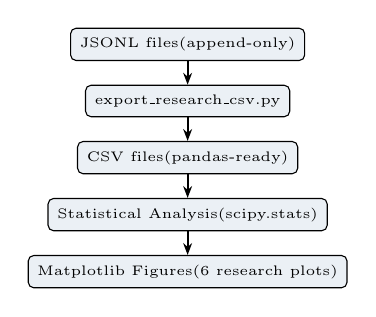
\begin{tikzpicture}[
  node distance=0.3cm,
  box/.style={rectangle, draw, rounded corners=2pt, font=\tiny, minimum width=2.0cm, minimum height=0.4cm, fill=ecublue!8},
  arrow/.style={-{Stealth[length=1.5mm]}, thick},
]
\node[box] (jsonl) {JSONL files\\(append-only)};
\node[box, below=of jsonl] (export) {export\_research\_csv.py};
\node[box, below=of export] (csv) {CSV files\\(pandas-ready)};
\node[box, below=of csv] (analysis) {Statistical Analysis\\(scipy.stats)};
\node[box, below=of analysis] (figs) {Matplotlib Figures\\(6 research plots)};

\draw[arrow] (jsonl) -- (export);
\draw[arrow] (export) -- (csv);
\draw[arrow] (csv) -- (analysis);
\draw[arrow] (analysis) -- (figs);
\end{tikzpicture}
\end{center}

\vspace{6pt}
\footnotesize
\textbf{Analysis Scripts:}
\begin{itemize}\scriptsize
  \item \texttt{run\_statistical\_analysis.py}: Pearson, paired tests
  \item \texttt{compute\_baseline.py}: Random, time, activity baselines
  \item \texttt{run\_sensitivity\_analysis.py}: 27 weight perturbations
  \item \texttt{visualize\_research\_data.py}: 6 publication figures
  \item \texttt{analyze\_attention.py}: Attention log processing
\end{itemize}
\end{column}
\end{columns}
\end{frame}

% =====================================================================
% SLIDE 31: Limitations & Future Work
% =====================================================================
\begin{frame}{Limitations \& Future Work}
\begin{columns}[T]
\begin{column}{0.48\textwidth}
\textbf{Honest Limitations}

\vspace{4pt}
\footnotesize
\begin{tabular}{@{}p{2.2cm}p{4.5cm}@{}}
\toprule
\textbf{Limitation} & \textbf{Impact} \\
\midrule
Sample size ($N{=}30$) & Limits generalizability; pilot study scale \\[4pt]
Binary attention & 0/100 classification loses granularity; no ``partially distracted'' state \\[4pt]
LLM latency (99--112\,s) & Not real-time; batch generation only. Acceptable for study materials, not live interaction \\[4pt]
Single institution & Cultural/demographic bias possible \\[4pt]
Controlled setting & Real-world noise (lighting, multiple faces) untested \\[4pt]
Q4 quantization & Accuracy trade-off vs full-precision; occasional JSON parse failures \\
\bottomrule
\end{tabular}
\end{column}

\begin{column}{0.48\textwidth}
\textbf{Future Work}

\vspace{4pt}
\footnotesize
\begin{enumerate}\scriptsize
  \item \textbf{Larger study} ($N > 200$) across multiple institutions for generalizability

  \item \textbf{Continuous attention scoring} (0--100) using angular distance from center instead of binary thresholding

  \item \textbf{Smaller LLMs}: Phi-3-mini (3.8B) or Gemma-2B for sub-30s generation on same hardware

  \item \textbf{Multimodal fusion}: Combine DSP scroll score + Vision attention into single engagement metric with learned weights

  \item \textbf{Adaptive difficulty}: Use real-time engagement to adjust quiz difficulty (if engaged $\Rightarrow$ harder questions)

  \item \textbf{IIR filter exploration}: Butterworth/Chebyshev for higher-rate scroll sampling

  \item \textbf{Longitudinal study}: Track engagement--performance correlation over a full semester
\end{enumerate}
\end{column}
\end{columns}
\end{frame}

% =====================================================================
% SLIDE 32: Conclusion
% =====================================================================
\begin{frame}{Conclusion}
\begin{columns}[T]
\begin{column}{0.32\textwidth}
\begin{block}{\centering DSP Results}
\begin{itemize}\scriptsize
  \item 9-stage pipeline: signal $\rightarrow$ score
  \item Scroll engagement $r = 0.866$\\($p < 0.001$, $N = 60$)
  \item DSP baseline $r = 0.834$ vs\\Random $r = 0.038$
  \item Weight sensitivity: $\sigma = 0.003$\\(stable under $\pm 10\%$)
\end{itemize}
\end{block}
\end{column}

\begin{column}{0.32\textwidth}
\begin{block}{\centering Vision Results}
\begin{itemize}\scriptsize
  \item solvePnP + Rodrigues pipeline
  \item Attention--quiz $r = 0.773$\\($p < 0.001$, $N = 120$)
  \item 3{,}857 frames analyzed
  \item MA filter reduces false\\positives (buffer = 10)
  \item CPU-only: no GPU contention
\end{itemize}
\end{block}
\end{column}

\begin{column}{0.32\textwidth}
\begin{block}{\centering System}
\begin{itemize}\scriptsize
  \item Full edge deployment\\(RTX 3060 + Ryzen 7)
  \item \textbf{Zero cloud egress}\\(Wireshark verified)
  \item 25+ API endpoints
  \item 7-table SQLite schema
  \item LLM: 99--112\,s (batch)
  \item Analytics: $< 200$\,ms (real-time)
\end{itemize}
\end{block}
\end{column}
\end{columns}

\vspace{8pt}
\begin{center}
\fbox{\parbox{0.85\textwidth}{\centering\footnotesize
\textbf{Objective Fulfilled:} We designed and evaluated an edge-deployed multimodal learning analytics system that applies DSP to scroll telemetry ($r = 0.866$) and CV-based head pose estimation ($r = 0.773$) to quantify student engagement and correlate it with academic performance --- all on consumer hardware with zero cloud dependency.
}}
\end{center}
\end{frame}

% =====================================================================
% END
% =====================================================================
\end{document}
